\newpage


\section{Domain Network Service}

\subsection{Definition}

Wikipeadia defines DNS as follows:
he Domain Name System (DNS) is a system used to convert a computer's host name into an IP address on the Internet.



\subsection{Configuration DNS Server}



Gabl /Weissenbach\newline

We installed the Server-roll "DNS" on the (R010) Win 2012 Server.

Finally, start the DNS Manager under Tools / DNS in Server Manager.
There we have selected the point Reverse Lookupzonen and in the context menu the point New Zone. These settings were made individually for each Vlan.\newline


\begin{minipage}[X]{0.8\textwidth} 
	\centering 
		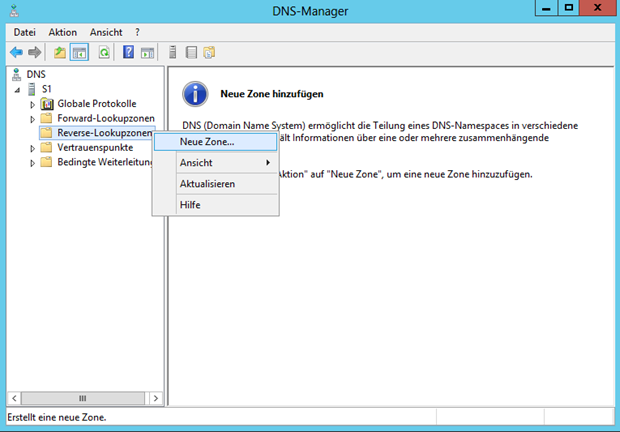
\includegraphics [scale=0.5]{graphics/1.png}
	\label{ecoconcept} 
\end{minipage} 
\newline\newline
We clicked through the welcome menu and selected Primary Zone.
\newline


\begin{minipage}[X]{0.8\textwidth} 
	\centering 
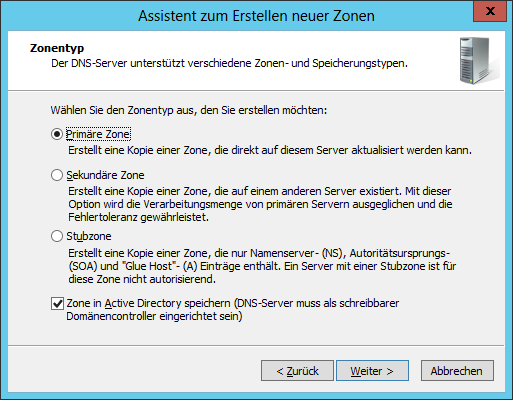
\includegraphics [scale=0.6]{graphics/2.png}
	\label{ecoconcept} 
\end{minipage} 


\begin{minipage}[X]{0.8\textwidth} 
	\centering 
	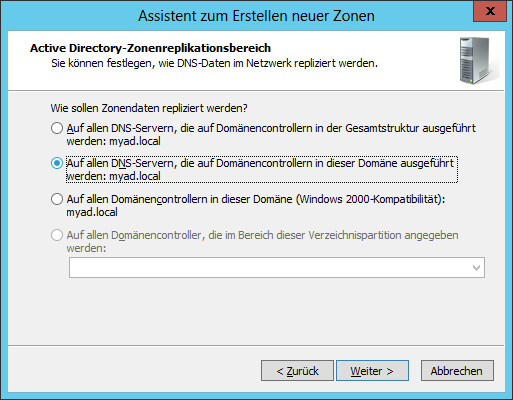
\includegraphics [scale=0.6]{graphics/3.png}	
	\label{ecoconcept} 
\end{minipage} \newline


Because it is an IPv4 network, we selected the IPv4 reverse lookup zone.\newline


\begin{minipage}[X]{0.8\textwidth} 
\centering 
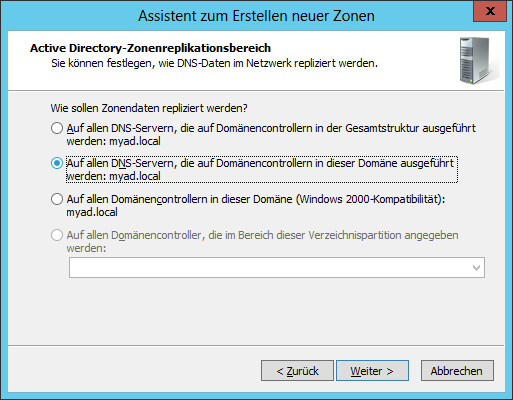
\includegraphics [scale=0.6]{graphics/4.png}
\label{ecoconcept} 
\end{minipage} \newline



Now we have specified the respective VLan. For this the fixed parts of the network address, as indicated in the screenshot.



We have retained the default setting for Dynamic Updates.\newline


\begin{minipage}[X]{0.8\textwidth} 
	\centering 
	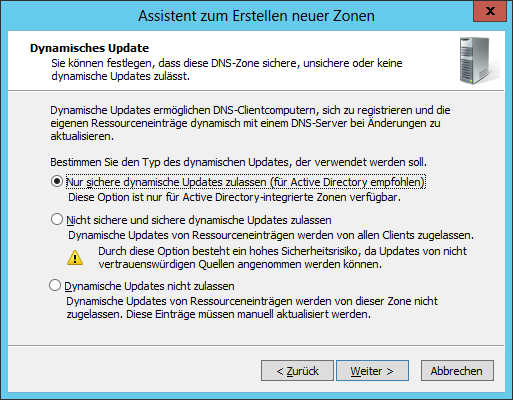
\includegraphics [scale=0.6]{graphics/5.png}
	\label{ecoconcept} 
\end{minipage} \newline

The DNS server, which is responsible for the respective VLAN, was informed of this. In order to resolve external addresses as well, a forwarding of the DNS queries must be created.\newline


\begin{minipage}[X]{0.8\textwidth} 
	\centering 
	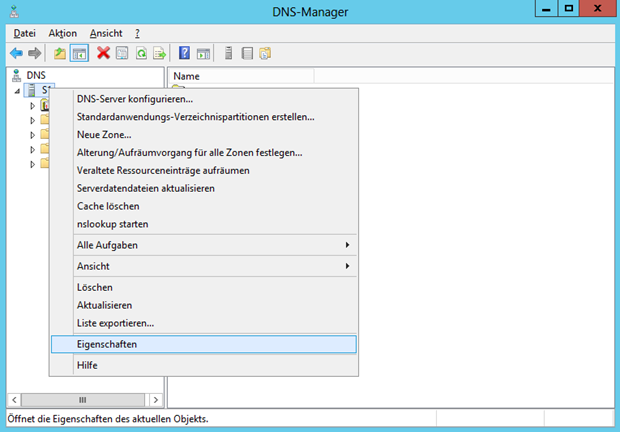
\includegraphics[scale=0.6]{graphics/6.png}  
	\label{ecoconcept} 
\end{minipage} \newline


In the IP settings of the clients on the network, the DNS server must be entered as the primary DNS server.\newline
